\documentclass[a4paper,12pt]{article}

% Pacotes
\usepackage[utf8]{inputenc}
\usepackage[brazil]{babel}
\usepackage{geometry}
\usepackage{graphicx}
\usepackage{amsmath}
\usepackage{hyperref}
\usepackage{verbatim}
\usepackage{float} 
\geometry{margin=2.5cm}
\graphicspath{{images/}}
\title{Projeto de Banco de Dados}
\author{
Yuri \\ Matrícula: 24.2.8116
\and
Bruno \\ Matrícula: XXXXX
}
\begin{document}

\maketitle

\tableofcontents
\newpage

\section{Introdução}

Este projeto tem como objetivo o desenvolvimento de um sistema de gerenciamento de torneios esportivos, com foco inicial em competições de futebol. O sistema permitirá a criação e administração de equipes, bem como a organização da tabela do campeonato.

A proposta visa estruturar e armazenar informações relevantes, como times participantes, partidas, resultados e classificação, utilizando um banco de dados relacional. Dessa forma, busca-se garantir maior eficiência, integridade e facilidade no gerenciamento das informações do torneio.

Inicialmente, o escopo do sistema será voltado para torneios de futebol, podendo ser expandido futuramente para outras modalidades esportivas.

\section{Objetivo}
O sistema tem como objetivo principal:
\begin{itemize}
    \item Descrever o problema
    \item Apresentar a solução proposta
    \item Organizar os dados de forma estruturada
\end{itemize}

\section{Requisitos do Sistema}

\subsection{Requisitos Funcionais}
\begin{itemize}
    \item Criar torneios
    \item Gerenciar esse torneio
    \item Gerenciar times
\end{itemize}

\subsection{Requisitos Não Funcionais}
\begin{itemize}

    \item Criptografia de CPF
\end{itemize}

\section{Modelo Conceitual}
Descreva o modelo entidade-relacionamento (ER).

\begin{figure}[H]
  \centering
  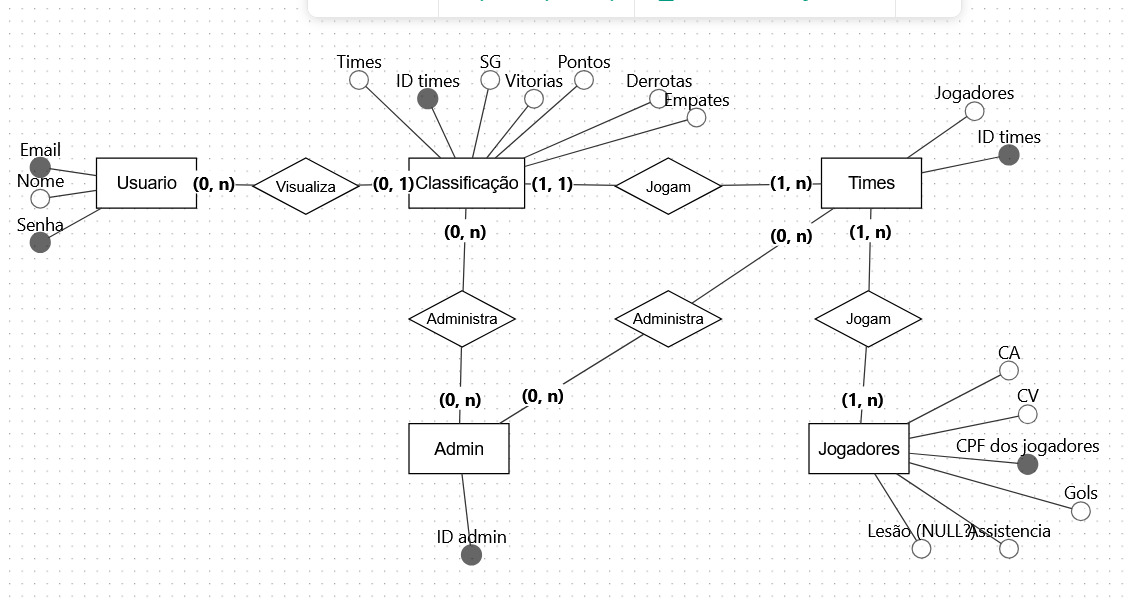
\includegraphics[width=1\textwidth]{Sem título.jpg}
   \caption{Modelo Conceitual}
\end{figure}

\begin{comment}
\section{Modelo Lógico}
Descreva as tabelas e seus relacionamentos.
\subsection{Tabela Usuário}

\begin{itemize}
    \item id (PK)
    \item nome
    \item email
\end{itemize}

\subsection{Tabela Livro}
\begin{itemize}
    \item id (PK)
    \item titulo
    \item autor
\end{itemize}

\subsection{Tabela Empréstimo}
\begin{itemize}
    \item id (PK)
    \item id\_usuario (FK)
    \item id\_livro (FK)
    \item data\_emprestimo
\end{itemize}
\end{comment}
\section{Modelo Físico}
Aqui você pode colocar o SQL:
\begin{comment}


\begin{verbatim}
CREATE TABLE Usuario (
    id INT PRIMARY KEY,
    nome VARCHAR(100),
    email VARCHAR(100)
);

CREATE TABLE Livro (
    id INT PRIMARY KEY,
    titulo VARCHAR(100),
    autor VARCHAR(100)
);

CREATE TABLE Emprestimo (
    id INT PRIMARY KEY,
    id_usuario INT,
    id_livro INT,
    FOREIGN KEY (id_usuario) REFERENCES Usuario(id),
    FOREIGN KEY (id_livro) REFERENCES Livro(id)
);
\end{verbatim}
\end{comment}
\section{Tecnologias Utilizadas}

\subsection{Linguagem de Programação}
O sistema será desenvolvido utilizando a linguagem Python, devido à sua simplicidade e ampla utilização no desenvolvimento de aplicações.

\subsection{Banco de Dados}
Será utilizado o Postgresql como sistema gerenciador de banco de dados, com modelagem relacional para garantir integridade e consistência dos dados.

\subsection{Interface}
A interface do sistema poderá ser desenvolvida como:
\begin{itemize}
    \item WEB?
    \item Interface?
\end{itemize}

\subsection{Ferramentas}
\begin{itemize}
    \item Postgresql
    \item GitHub
\end{itemize}
\section{Conclusão}
Apresente os resultados obtidos e possíveis melhorias futuras.

\end{document}